\documentclass[11pt,border=6pt]{standalone}
\usepackage{fontspec}
\usepackage{tikz}
\usetikzlibrary{positioning,arrows.meta,calc,shapes.multipart}
\begin{document}
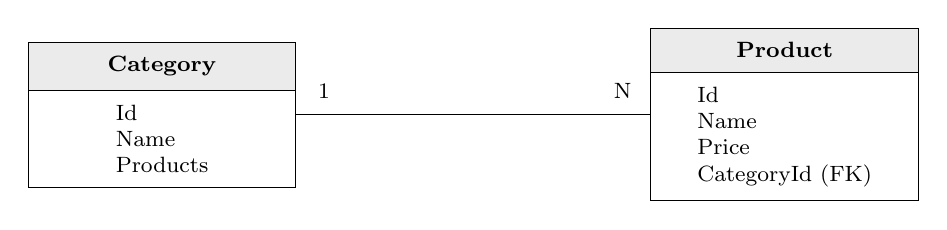
\begin{tikzpicture}[font=\footnotesize,
  entity/.style={draw, rectangle split, rectangle split parts=2,
    rectangle split part fill={black!8,white}, align=left, inner sep=5pt,
    minimum width=3.4cm, font=\footnotesize},
  rel/.style={semithick}]

  \node[entity] (cat) at (0,0) {\textbf{Category}\nodepart{second}Id\\Name\\Products};
  \node[entity, anchor=west] (prod) at (6.2,0) {\textbf{Product}\nodepart{second}Id\\Name\\Price\\CategoryId (FK)};

  \draw[rel] (cat.east) -- (prod.west |- cat.east);
  \node[font=\footnotesize, above=1pt] at ($(cat.east)+(0.35,0.05)$) {1};
  \node[font=\footnotesize, above=1pt] at ($(prod.west)+(-0.35,0.05)$) {N};
\end{tikzpicture}
\end{document}

